\documentclass[xcolor=dvipsnames]{beamer}
\usepackage[T1]{fontenc}
\usepackage{fontenc}
\usepackage{textcomp}
\usepackage{lmodern}
\usepackage[utf8]{inputenc}
\usepackage{xcolor}
\usepackage{graphicx}
\usepackage{MnSymbol}
\usepackage{stmaryrd}
\usepackage{colortbl}
\usepackage{caption}
\usepackage{comment}
\usepackage{pdfpages}
\usepackage{booktabs}
\usepackage{soul}
\usepackage[normalem]{ulem}


\usepackage{tcolorbox}
\usepackage{lipsum}


%%%%%%%%%%%%%%%%%%%%%%%%%%%%%%%%%%%%%%%%%%%%%%%%%

\usepackage{pgf}
\usepackage{etex}
\usepackage{tikz,pgfplots}


\usetheme{Antibes}
%\usetheme{Madrid}
%\usecolortheme[named=Maroon]{structure}
\usecolortheme{dolphin}
\usefonttheme{professionalfonts}
\useoutertheme{infolines}
\useinnertheme{circles}

\newtheorem*{bem}{Bemerkung}

\usepackage{tikz}


%%%%%%%%%%%%%%%%%%%%%%%%%%%%%%%%%%%%%%%%%%%%%%%%%



%%%%%%%%%%%%%%%%%%%%%%%%%%%%%%%%%%%%%%%%%%%%%%%%%
\usepackage{listings}
\usepackage{color}

\definecolor{dkgreen}{rgb}{0,0.6,0}
\definecolor{gray}{rgb}{0.5,0.5,0.5}
\definecolor{mauve}{rgb}{0.58,0,0.82}
\definecolor{mymauve}{rgb}{0.58,0,0.82}
\lstset {
  basicstyle=\footnotesize,        % size of fonts used for the code
  breaklines=true,                 % automatic line breaking only at whitespace
  captionpos=b,                    % sets the caption-position to bottom
  commentstyle=\color{mygreen},    % comment style
  escapeinside={\%*}{*)},          % if you want to add LaTeX within your code
  keywordstyle=\color{blue},       % keyword style
  stringstyle=\color{mymauve},     % string literal style
  tabsize=2,
  showstringspaces=false
}

\definecolor{lightgray}{rgb}{.9,.9,.9}
\definecolor{darkgray}{rgb}{.4,.4,.4}
\definecolor{purple}{rgb}{0.65, 0.12, 0.82}


\lstdefinelanguage{JavaScript}{%
  keywords={const, let, typeof, instanceof, new, true, false, catch, function, return, null, undefined, catch, switch, var, if, in, while, for, do, else, case, break},
  keywordstyle=\bfseries,
  ndkeywords={class, export, throw, import, this},
  ndkeywordstyle=\bfseries,
  sensitive=false,
  comment=[l]{//},
  morecomment=[s]{/*}{*/},
  commentstyle=\ttfamily,
  stringstyle=\color{blue}\ttfamily,
  morestring=[b]',
  morestring=[b]`,
  morestring=[b]"
}


%%%%%%%%%%%%%%%%%%%%%%%%%%%%%%%%%%%%%%%%%%%%%%%%%


\title[Introduzione a Redis]{REDIS}
\subtitle[Open source in-memory data structure store]{Open source in-memory data structure store}
\author[Riciputi Jacopo]{Riciputi Jacopo}
  \logo{
\includegraphics[height=0.5cm]{res/redisLogo.png}}
\date{30 Maggio 2018}
\logo{\pgfimage[height=0.8cm]{res/redisLogo.png}}

\begin{document}

\begin{frame}
  \titlepage
\end{frame}

\begin{frame}
\frametitle{Indice}
\tableofcontents
\end{frame}

  \section{Redis}
    \subsection{Cos'è}
      \begin{frame}{Cos'è}
          \textbf{Redis} è uno store di strutture dati completamente in-memory, prestante e open source. \\
          È utilizzato principalmente come:
          \begin{itemize}
            \item Database;
            \item Cache;
            \item Message broker.
          \end{itemize}
          Soprattutto per:
          \begin{itemize}
            \item applicazioni Web;
            \item videogiochi;
            \item sistemi IoT.
          \end{itemize}

          Tra i punti di forza vi sono \textbf{velocità} e la \textbf{facilità} con cui permette di gestire varie strutture dati.
          %come stringhe, hash, liste, set e sorted set, bitmaps, hyperloglogs e indici geospaziali interrogabili tramite query dedicate.
      \end{frame}

      \begin{frame}{Perchè è uno dei più utilizzati}
        Nel mondo di database NoSQL Redis risulta essere il secondo database NoSQL, alle spalle del colosso
        MongoDB e in 7 posizione se vengono considerati anche i database relazionali.\footnote{\url{https://db-engines.com/en/ranking}} \\
        Tra i suoi \textbf{punti di forza}:
        \begin{itemize}
          \item La struttura chiave-valore permette di gestire più strutture dati;
          \item Il mantenimento dei dati in memoria ed il linguaggio in cui è scritto (C) lo rendono \textbf{estramente veloce}
                e con tempi di latenza minimi;
          \item Opzionalmente è permette di aggiungere \textbf{persistenza};
          \item Supporta le transazioni;
          \item Fornisce funzionalità per eseguire \textbf{Lua scripting}, grazie ad un interprete built-in;
          \item Offre \textbf{high avalability} e supporta la suddivisione dei dati all'interno di una rete \textbf{cluster} di macchine.
        \end{itemize}

      \end{frame}

      \begin{frame}{Estramente veloce}
        \begin{center}
        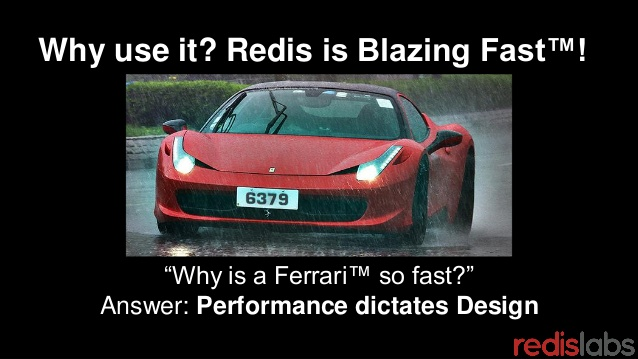
\includegraphics[height=6.cm]{res/redisFerrari.jpg}
        \end{center}
      \end{frame}


  \section{Primi passi}
      \begin{frame}
        \begin{block}{\centering \huge \insertsectionhead}
        \end{block}
      \end{frame}
      \subsection{Get started}
        \begin{frame}{Primi Passi}
          Installare Redis richiede qualche semplice passo se scaricato dalla pagina ufficiale\footnote{\url{https://redis.io/download}} oppure è possibile ottenere una versione completa su Debian o derivate lanciando il comando \textbf{\textit{sudo apt-get install redis-server}}.\\

          \begin{itemize}
            \item Una volta installato, con il comando \textbf{\textit{redis-server}} viene avviata un'instanza sulla porta di defalut (6379)
            \item È possibile collegarsi da terminale a questa instanza tramite il client \textbf{\textit{redis-cli}}
          \end{itemize}

          A questo punto si è completamente operativi.\\
          \textbf{Esempio base:}\\
          Redis per la gestione di semplici chiavi fornisce i comamdi \textbf{SET} e \textbf{GET}
          \begin{itemize}
            \item \textbf{SET} richiede una chiave e il corrispettivo valore.\\ Es. SET foo bar $\rightarrow$ OK
            \item \textbf{GET} Data una chiave ne ritorna il valore. Es. GET foo $\rightarrow$ bar
          \end{itemize}
        \end{frame}

      \subsection{Strutture Dati}
        \begin{frame}{Strutture Hash}
          \textbf{HSET} consente di creare una chiave a cui associare più coppie chiave-valore. \\
          > HSET hfoo firstKey firstValue \\
          (integer 1)\\
          > HSET hfoo secondKey secondValue\\
          (integer 1)

          \bigskip

          È possibile riottenere questi valore in differenti modi:
          \begin{itemize}
            \item HGET hfoo firstKey $\rightarrow$ "firstValue"
            \item HGETALL hfoo \\
                  1) "firstKey"
                  2) "firstValue"
                  3) "secondKey"
                  4) "secondValue"
            \item E' possile altrimenti ottenere tutte le chiavi o tutti i valori rispettivamente con i comandi \textbf{HKEYS} e  \textbf{HVALS}
          \end{itemize}

        \end{frame}

\begin{frame}[fragile]
  \frametitle{Liste}
  Redis offre la possibilità di gestire le liste, tramite i comandi \textbf{LPUSH} e \textbf{LPOP} per le operazioni in testa,
  \textbf{RPUSH} e \textbf{RPOP} per quelle in coda.
  \\
  \begin{lstlisting}[language=bash]
    > LPUSH list 2
    (integer) 1
    > RPUSH list 3
    (integer) 2
    > LPUSH list 1
    (integer) 3
  \end{lstlisting}

  Redis restituirà i valori in ordine "1", "2", "3". \\
  È possibile verificarlo con l'istruzione \textbf{LRANGE}
  \\

  \begin{lstlisting}[language=bash]
    > LRANGE list 0 -1
    1) "1"
    2) "2"
    3) "3"
  \end{lstlisting}

\end{frame}

\begin{frame}[fragile]{Set}
  Nella gestione dei set in Redis si possiedono due comandi principali, \textbf{SADD} e \textbf{SMEMBERS},
  rispettivamente per aggiungere valori ad una chiave e visualizzare i suoi elementi.
  \begin{lstlisting}[language=bash]
    > SADD myset 1 2 3
    ( integer ) 3
    > SMEMBERS myset
    1. "3"
    2. "1"
    3. "2"
  \end{lstlisting}

  Decisamente più interessanti i \textbf{Sordet Set}.


\end{frame}

\begin{frame}[fragile]{Sorted Set}
  Questa struttura dati è gestita da Redis associando ad ogni valore uno \textit{score}.
  \\
  L'ordinamento viene infatti eseguito in base al valore di questo \textit{score}.\\
  Se per due valori coincide sarà eseguito sul valore lessicografico di quest'ultimi.
  \\
  In questo caso i comandi base sono:
  \begin{itemize}
    \item \textbf{ZADD}: Prende in ingresso chiave, score e valore e li immaggazzina
    \item \textbf{ZRANGE}: Data una chiave, indice di partenza e di fine ne visualizza in ordine \textbf{crescente} i valori;
    \item \textbf{ZREVRANGE}: Data una chiave, indice di partenza e di fine ne visualizza in ordine \textbf{decrescente} i valori;
    \item \textbf{ZRANGEBYLEX}, \textbf{ZREVRANGEBYLEX}, \textbf{ZREMRANGEBYLEX} e \textbf{ZLEXCOUNT} per manipolarli in base al valore lessicografico.
  \end{itemize}

\end{frame}

\begin{frame}[fragile]{Sorted Set}
  \begin{lstlisting}[language=bash]
    > ZADD classe 1996 "Mario Rossi"
    ( integer ) 1
    > ZADD classe 1993 "Fabio Bianchi"
    ( integer ) 1
    > ZADD classe 1987 "Roberto Verdi"
    ( integer ) 1
    > ZADD classe 1990 "Carlo Neri"
    ( integer ) 1

    > ZRANGE classe 0 -1
    1) "Roberto Verdi"
    2) "Carlo Neri"
    3) "Fabio Bianchi"
    4) "Mario Rossi"
  \end{lstlisting}
\end{frame}

\subsection{Nodejs client}
\begin{frame}[fragile]{Nodejs client}
  \textbf{npm install ioredis} - Client molto semplice per Nodejs \\
  \begin{lstlisting}[language=JavaScript]
      var Redis = require("ioredis");
      var redis = new Redis({
        port: 6379,
        host: "127.0.0.1",
        family: 4,
      });

      redis.set("foo", "bar");
      redis.get("foo", function(err, result) {
        console.log(result);
      });

      redis.del("foo");
      redis.get("foo", function(err, result) {
        console.log(result);
      });
  \end{lstlisting}

\end{frame}

\begin{frame}[fragile]{Nodejs client}
  Output:
  \begin{lstlisting}[language=bash]
    bar
    null
  \end{lstlisting}

  Qualcosa di più "complicato":
  \begin{lstlisting}[language=JavaScript]
    redis.hmset("me",
                "name","jacopo",
                "surname", "riciputi",
                "age", 22);

    redis.hgetall("me", function(err, result){
        console.log(result);
    });

    Output:
    { name: 'jacopo', surname: 'riciputi', age: '22'}
  \end{lstlisting}
\end{frame}


\section{Utilizzo}
  \begin{frame}
    \begin{block}{\centering \huge \insertsectionhead}
    \end{block}
  \end{frame}
  \subsection{Caching}
    \begin{frame}{Caching}
      \textbf{Problemi:}
        \begin{itemize}
          \item Difficoltà nella digestione dei dati;
          \item Mobile, IoT, web 2.0 producono continuamente informazioni;
          \item Impossibile eseguire processi real-time.
        \end{itemize}

      \textbf{Soluzione} $\rightarrow$ Pulire i dati con Redis!!
      \begin{center}
      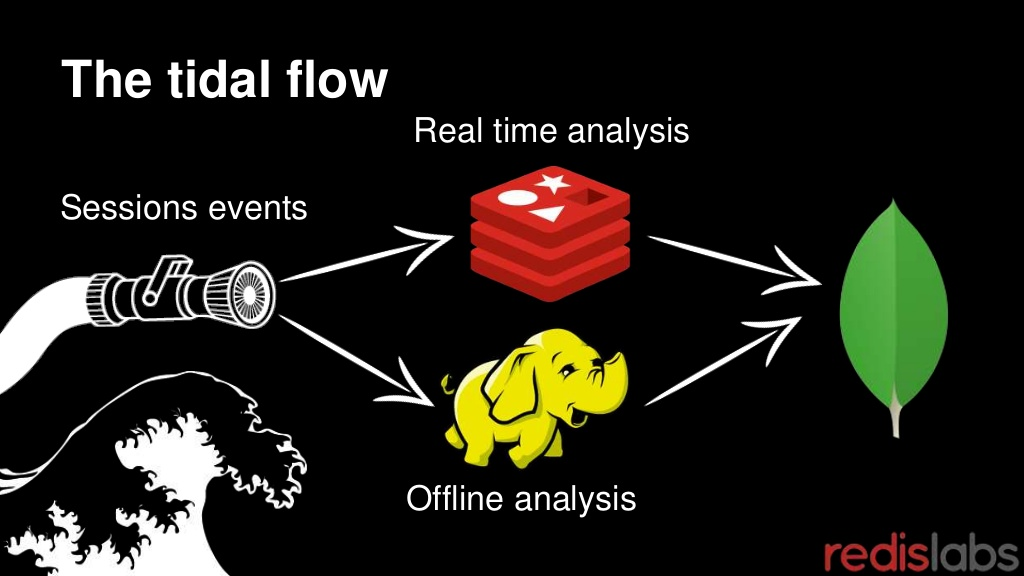
\includegraphics[height=4.cm]{res/realTimeRedis.jpg}
      \end{center}
    \end{frame}

    \begin{frame}{Caching}
      L'idea è di accompagnare la sessione dell'utente con Redis.
      \\
      Al suo termine i dati saranno processati, "ripuliti" e passati a contenitori più grandi (es. MongoDB) \\
      Le sessioni terminano dopo un logout o un timeout.
      \begin{itemize}
        \item \textbf{Facile} identificare il logout
        \item \textbf{Difficile} rilevare un timeout, soprattutto considerando le migliaia di sessioni che possono essere attive
      \end{itemize}
      \bigskip
      \textbf{Qui Redis viene in soccorso!}
      \\
      Permette infatti di associare una scadenza alle chiavi e di gestirne le notifiche.
    \end{frame}

    \subsection{Message Broker}
    \begin{frame}{Message Broker}
      Redis offre la possibilità di gestire un \textbf{PUB/SUB messaging paradigm}. \\
      Sarà possibile perciò client iscritti ad un determinato canale ed publisher che inviano messaggi.
      Ogni emittente non è programmato per inviare ad uno specifico destinatario ma a tutti i subscriber di un determinato canale.
      \begin{itemize}
        \item Iscrizione con \textbf{SUBSRIBE foo}
        \item Publicazione con \textbf{PUBLISH foo hello}
        \item È possibile sottoscriversi utilizzando i pattern con \textbf{PSUBSCRIBE h?llo} \\
              Accetterà messaggi da hello, hallo, hxllo ma non da hllo.
      \end{itemize}
    \end{frame}

    \subsection{Database}
      \begin{frame}{Database}
          Il mondo odierno necessita di analisi istantanee, i tradizionali tool necessitano ore, se non giorni! \\
          Redis offre: \\
          \begin{itemize}
            \item Analisi in tempo reale;
            \item Transazioni atomiche;
            \item Supporto ad un elevatissimo numero di transazioni per secondo;
            \item L'assenza di struttura e la semplicità nella modellazione dei dati lo rende un valido elemento come base di un backend web.
            \item È possibile scalare le dimensioni dell'applicazione aggiungendo macchine in una rete cluster.
          \end{itemize}
      \end{frame}

    \section{Casi d'uso}
      \begin{frame}
        \begin{block}{\centering \huge \insertsectionhead}
        \end{block}
      \end{frame}
      \subsection{Clash of Clans}
        \begin{frame}{Clash of Clans}
          \begin{itemize}
            \item Gioco real-time con milioni di utenti.
            \item Il datastorage principale è MongoDB.
            \item Utilizza Redis per il salvataggio e la progressione delle partite.
            \item Nel dettaglio per l'aggiornamento delle risorse real-time, i punteggi e le classifiche.
          \end{itemize}
          \begin{center}
          
\includegraphics[height=3.cm]{res/clash.png}
          \end{center}
        \end{frame}

        \subsection{Waze}
          \begin{frame}{Waze}
            \begin{itemize}
              \item Focus sul traffico real-time
              \item Più di 10 milioni di utenti collegati nelle ore di punta
              \item Database principale: MongoDB.
              \item Utilizza Redis per gli aggiornamenti in tempo reale sul traffico, i veicoli e i passeggeri. \\
                    I dati venono appoggiati al suo interno per poi periodicamente elaborati per \textbf{aggiustamenti} e \textbf{notifiche}.
            \end{itemize}



            \begin{center}
            
\includegraphics[height=2.cm]{res/waze.png}
            \end{center}
          \end{frame}

      \section{Conclusioni}
        \begin{frame}
          \begin{block}{\centering \huge \insertsectionhead}
          \end{block}
        \end{frame}
        \begin{frame}{In sintesi}
          \begin{itemize}
            \item Prestazioni e facilità d'uso;
            \item Molteplici strutture dati;
            \item Scalabilità;
            \item Forte community, driver per molti linguaggi;
            \item Vari scenari: Caching, Message Broker, Database;
            \item Open source ed estendibile: RediSearch / rediSQL / ReJSON / Redis Graph;
            \item Cuore italiano ! \footnote{\url{https://github.com/antirez}}
          \end{itemize}
          \begin{center}
          
\includegraphics[height=2.cm]{res/italy.jpg}
          \end{center}
        \end{frame}



%%%%%%%%%%%%%%%%%%%%%%%%%%%%%%%%%%%%%%%%%%%%%%%%%%%
\end{document}
